\documentclass[aspectratio=169,11pt]{beamer}

% ---- Theme ----
\usetheme{metropolis}
\metroset{block=fill, sectionpage=none, numbering=fraction}
\usepackage{appendixnumberbeamer}
\usepackage{booktabs}
\usepackage{graphicx}
\usepackage{listings}

% ---- Accent colours (defined BEFORE lstset, which references softGrey) ----
\definecolor{accentBlue}{HTML}{2C6E9B}
\definecolor{accentAmber}{HTML}{C9810A}
\definecolor{accentRed}{HTML}{B23A3A}
\definecolor{softGrey}{HTML}{F2F2F0}
\setbeamercolor{frametitle}{bg=accentBlue}

\lstset{basicstyle=\ttfamily\scriptsize, breaklines=true,
  columns=fullflexible, backgroundcolor=\color{softGrey},
  frame=none, xleftmargin=2pt, xrightmargin=2pt}

% ---- Additions (not in the original template) ----
\usepackage{tabularx}
\usepackage{array}
\newcolumntype{L}{>{\raggedright\arraybackslash}X}
\setbeamercolor{alerted text}{fg=accentAmber}
\setbeamercolor{block title}{bg=accentBlue!15, fg=accentBlue}
\newcommand{\src}[1]{{\scriptsize\color{white!75!accentBlue}#1}}

% ---- Additions for this deck ----
\usepackage{tikz}
\usetikzlibrary{positioning, arrows.meta}
\definecolor{doneGreen}{HTML}{2E7D4F}
\newcommand{\done}{{\small\color{doneGreen}\textbf{done}}}
\newcommand{\now}{{\small\color{accentAmber}\textbf{in progress}}}
\newcommand{\todo}{{\small\color{gray}\textbf{planned}}}
\newcommand{\fine}[1]{{\scriptsize\color{gray}#1}}
% Speaker notes: hidden in the PDF by default.
% To print them, replace the next line with: \setbeameroption{show notes on second screen=right}
\setbeameroption{hide notes}

\title{AgentVerify 2027: Paper Roadmap}
\subtitle{Requirement-related failures in coding-agent runs}
\author{Cris Huynh \quad (with Phin)}
\institute{Ontario Tech University \quad\textbullet\quad Supervisors: Dr.\ Kundi Yao, Dr.\ Sanaa Alwidian}
\date{September 2026}

\begin{document}

% =====================================================================
\maketitle
\note{Short roadmap: what the paper is about, where RQ1 stands, what comes next.}

\begin{frame}{Roadmap}
  \begin{enumerate}
    \item Introduction: problem, gap, motivation
    \item Data and studies
    \item Research questions \hfill {\small RQ1 \now}
    \item RQ1 progress: what, why, how
    \item What we expect from RQ1
    \item How RQ1 leads to RQ2 and RQ3
    \item Plan for this week and to the deadline
  \end{enumerate}
  \vfill
  \fine{Target: AgentVerify 2027 workshop (co-located with ICSE 2027). Abstract Nov 1, paper Nov 6 (AoE).}
\end{frame}

% =====================================================================
\section{Introduction}

\begin{frame}{The problem: a bridge to the wrong island}
  \begin{columns}[T]
    \begin{column}{0.5\textwidth}
      \begin{block}{Analogy}
        A builder is asked for a bridge to \textbf{Island A}.\\
        The bridge is strong, no cracks, no alarms.\\
        It goes to \textbf{Island B}.\\[4pt]
        Only the \alert{contract} shows the failure.
      \end{block}
    \end{column}
    \begin{column}{0.5\textwidth}
      \begin{block}{Real agent run}
        Task: \emph{``use the Qwen2.5 tokenizer''}\\
        Agent: used \textbf{Qwen2}.\\
        No error, no failing command, clean output.\\[4pt]
        The answer is simply \alert{wrong}.
      \end{block}
    \end{column}
  \end{columns}
  \vfill
  \centering Monitors that wait for an error, crash or failing test \textbf{may never see} this kind of failure.
  \note{Tell the bridge story first. Then the Qwen example (count-dataset-tokens, terminus2, gemini). Message: a requirement failure can look perfectly healthy from the inside.}
\end{frame}

\begin{frame}{The gap}
  \begin{itemize}
    \item \textbf{Failure as a Process} (FaaP; Zhao et al.) studies \emph{how} coding-agent failures unfold:
      when the mistake happens, when the run is lost, when a signal first appears.
    \item FaaP's own monitor experiment hints that requirements matter:
      giving the monitor the task's requirements raised detection of \emph{specification neglect}
      from \textbf{3\% to 22\%}.
    \item But no study, to our knowledge, asks whether \textbf{requirement-related failures unfold differently}
      from other failures, using a requirement label that is \textbf{checked against the task text}.
  \end{itemize}
  \vfill
  \fine{3\%$\rightarrow$22\%: FaaP replication package, \texttt{docs/oracle\_VARIANTS.md}. Gap kept modest on purpose.}
  \note{Kundi's advice: keep the gap modest and cover the relevant papers. We do not claim nobody studies requirement failures; we claim nobody compares their timing and visibility with a checked requirement label.}
\end{frame}

\begin{frame}{Motivation}
  \begin{block}{If requirement failures stay silent more often\dots}
    \dots then waiting for an alarm is not enough.\\
    A monitor must \textbf{read the requirement} (the contract) to catch them.
  \end{block}
  \vspace{6pt}
  \begin{itemize}
    \item Early hint in FaaP's own labels: runs labeled \emph{specification neglect} end silent in
      \textbf{44\%} of cases, vs \textbf{28\%} of all failed runs.
    \item This hint uses FaaP's labels as-is. RQ1 re-tests it with a cleaner, checkable definition.
  \end{itemize}
  \vfill
  \fine{44.3\% = 78/176 runs; 28.0\% = 332/1,184 runs. Descriptive only, seen before the plan was written (disclosed).}
  \note{This is why we ask RQ1. Be clear that 44 vs 28 is a hint from FaaP's labels, not our result.}
\end{frame}

% =====================================================================
\section{Data and studies}

\begin{frame}{Data and studies}
  \small
  \begin{tabularx}{\textwidth}{@{}lLL@{}}
    \toprule
      & \textbf{Study 1: FaaP (Terminal-Bench)} \hfill \now & \textbf{Study 2: Nebius (GitHub issues)} \hfill \todo \\
    \midrule
    Runs & 1,794 runs (1,184 failed); 89 tasks, 3 agent frameworks, 7 models & $\sim$80,000 SWE-agent runs on $\sim$3,600 issues; we sample $\sim$200 failed runs \\
    Requirement & Original \texttt{task.yaml} text, pinned commit & GitHub issue text \\
    Timing labels & FaaP's (mistake, point of no return, first signal) & We create them (LLM draft + human check) \\
    ``Silent'' & FaaP's label (cannot be re-checked) & \textbf{A rule on the raw run}: any error, traceback or failing test before the end? \\
    \bottomrule
  \end{tabularx}
  \vfill
  \fine{Study 2 answers Kundi's request to go beyond one dataset, and removes our dependence on FaaP's unverifiable labels.}
  \note{Study 1 is big and fast because timing labels exist. Study 2 is smaller but fully checkable. If both agree, FaaP's messiness matters much less.}
\end{frame}

% =====================================================================
\section{Research questions}

\begin{frame}{Research questions}
  \begin{tabularx}{\textwidth}{@{}lLl@{}}
    \toprule
    & \textbf{Question} & \textbf{Status} \\
    \midrule
    \textbf{RQ1} & Do requirement-related failures differ from other failures in \textbf{when they start},
      \textbf{how long they stay fixable}, and \textbf{how often they stay silent}? & \now \\[4pt]
    \textbf{RQ2} & Can two people reliably find the step where a run stops following the requirement,
      using only the requirement text and the run (no test results)? & \todo \\[4pt]
    \textbf{RQ3} & How often do runs stop following the requirement, and does it also happen in runs that
      \textbf{pass} the tests? & \todo \\
    \bottomrule
  \end{tabularx}
  \vfill
  \fine{RQ2 and RQ3 wording to be confirmed; both use Nebius Draw 2 (20 runs, labeled by two raters, outcome kept in a sealed key file).}
  \note{RQ1 is the only one in progress. RQ2 and RQ3 follow from it (see the connection slide).}
\end{frame}

% =====================================================================
\section{RQ1 progress}

\begin{frame}{Why we cannot use FaaP's labels directly}
  \begin{columns}[T]
    \begin{column}{0.52\textwidth}
      FaaP labels every failure \textbf{twice}:
      \begin{itemize}
        \item \emph{trigger} (why): \texttt{spec\_neglect} \textbf{176} runs
        \item \emph{category} (what): names the requirement \textbf{251} runs
        \item \textbf{both}: only \textbf{116} \quad either: \textbf{311}
      \end{itemize}
      \vspace{4pt}
      Example: ``used Qwen2 instead of Qwen2.5'' is filed as \emph{false premise}.
    \end{column}
    \begin{column}{0.46\textwidth}
      \begin{block}{Requirements not in the text}
        \texttt{rare-mineral-allocation}: FaaP's largest \emph{spec neglect} task (17 runs).\\
        The task text \textbf{never} says where to write the answer; only the hidden test expects
        \texttt{/app/solution.txt}.
      \end{block}
    \end{column}
  \end{columns}
  \vfill
  \centering Like comparing patients with an unreliable diagnosis: \textbf{we redo the diagnosis first.}
  \note{The two FaaP fields disagree often. And part of FaaP's specification neglect is about expectations that are not in the specification. That is why labeling is the first half of RQ1.}
\end{frame}

\begin{frame}{RQ1 pipeline}
  \centering
  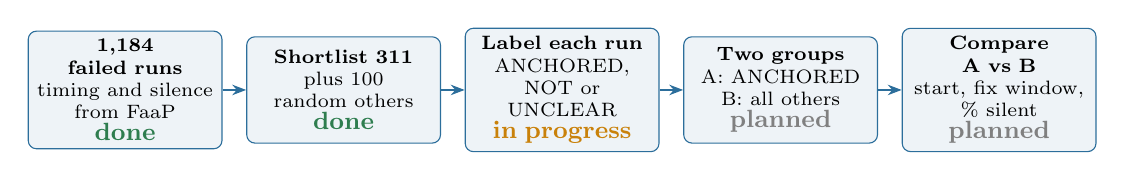
\begin{tikzpicture}[
      box/.style={draw=accentBlue, fill=accentBlue!8, rounded corners=3pt, align=center,
                  minimum height=1.35cm, text width=2.25cm, inner sep=3pt, font=\scriptsize, execute at begin node={\hyphenpenalty=10000\exhyphenpenalty=10000}},
      arr/.style={-{Stealth[length=5pt]}, thick, accentBlue}]
    \node[box] (a) {\textbf{1,184 failed runs}\\ timing and silence\\ from FaaP\\ \done};
    \node[box, right=0.3cm of a] (b) {\textbf{Shortlist 311}\\ plus 100\\ random others\\ \done};
    \node[box, right=0.3cm of b] (c) {\textbf{Label each run}\\ ANCHORED,\\ NOT or UNCLEAR\\ \now};
    \node[box, right=0.3cm of c] (d) {\textbf{Two groups}\\ A: ANCHORED\\ B: all others\\ \todo};
    \node[box, right=0.3cm of d] (e) {\textbf{Compare A vs B}\\ start, fix window,\\ \% silent\\ \todo};
    \draw[arr] (a) -- (b); \draw[arr] (b) -- (c); \draw[arr] (c) -- (d); \draw[arr] (d) -- (e);
  \end{tikzpicture}
  \vspace{10pt}
  \begin{itemize}\small
    \item The 100 random runs only \textbf{measure} how many requirement failures the shortlist misses; they do not join group A.
    \item Everything is scripted and reproducible: \texttt{scripts/step1\_*} to \texttt{step3\_*}; outputs are identical on rerun.
  \end{itemize}
  \note{Walk left to right. The measurements already exist (FaaP). Our work is the middle box: deciding who belongs in group A.}
\end{frame}

\begin{frame}{How one run is labeled}
  \begin{block}{One question}
    At the decisive mistake, did the agent \textbf{stop doing something the task text clearly asked for}?\\
    \textbf{Yes} $\rightarrow$ ANCHORED \quad \textbf{No}, it tried but failed for another reason $\rightarrow$ NOT \quad \textbf{Can't tell} $\rightarrow$ UNCLEAR
  \end{block}
  \begin{block}{Tie-breaker (the bridge test)}
    If the agent's own plan had worked perfectly, would the requirement be met?\\
    Plan targets Island B $\rightarrow$ ANCHORED. \quad Right plan, bad concrete $\rightarrow$ NOT.
  \end{block}
  \begin{itemize}\small
    \item \textbf{Only the task text counts.} Expected only by a hidden test $\rightarrow$ NOT, marked \emph{implicit}.
    \item Every ANCHORED label quotes the \textbf{exact words} of the task and of the evidence, so anyone can check it.
  \end{itemize}
  \note{Full rules: docs/labeling\_guide.md. The labeler never sees FaaP's labels, timing or silence, so labels cannot be steered toward the result.}
\end{frame}

\begin{frame}{Two examples}
  \small
  \begin{tabularx}{\textwidth}{@{}lLL@{}}
    \toprule
    & \textbf{ANCHORED} & \textbf{NOT} \\
    \midrule
    Run & \texttt{count-dataset-tokens} (terminus2, gemini) & \texttt{create-bucket} (miniswe, gpt5) \\
    Task text & ``You should use the Qwen2.5-1.5B-Instruct tokenizer'' & ``Create an S3 bucket named "sample-bucket" using the aws cli'' \\
    What happened & Used \texttt{Qwen/Qwen2-1.5B-Instruct} instead & Assumed real AWS credentials were needed; never found the local mock \\
    Bridge test & Plan targets another tokenizer: \textbf{requirement missed} & Plan targets the right bucket: \textbf{environment belief failed} \\
    \bottomrule
  \end{tabularx}
  \note{These two are fixed worked examples in the labeling guide and are not in Kundi's blind set.}
\end{frame}

\begin{frame}{How we keep it trustworthy}
  \begin{enumerate}
    \item \textbf{Drafts, not decisions.} Claude drafted every run twice, independently
      (the two passes agree on 92.7\%). Cris decides every label himself.
    \item \textbf{Second rater, blind.} Kundi labels 50 random runs without seeing any other labels.
      We report \% agreement and Cohen's $\kappa$ (target $\geq$ 0.61; if lower, fix the guide and relabel).
    \item \textbf{Freeze before numbers.} The plan is tagged in git before any group comparison.
      Anything changed later is reported as a change.
    \item \textbf{Honest limits.} FaaP's timing and silence labels cannot be re-checked (no raw runs released);
      their per-run agreement file could not confirm their reported agreement.
  \end{enumerate}
  \note{92.7\% is agreement between two AI passes: it shows the drafts are stable, not that they are right. The reliability number is Kundi vs Cris.}
\end{frame}

\begin{frame}{How we compare the two groups}
  \begin{columns}[T]
    \begin{column}{0.42\textwidth}
      \small
      \begin{tabular}{@{}lcc@{}}
        \toprule
        & \textbf{A} & \textbf{B} \\
        \midrule
        Median start step & ? & ? \\
        Median fix window & ? & ? \\
        \% silent & ? & ? \\
        \bottomrule
      \end{tabular}\\[8pt]
      \textbf{Is the gap real?} Redraw the 87 tasks 10,000 times; the gap's range must not include 0.
    \end{column}
    \begin{column}{0.56\textwidth}
      \small
      \begin{tabularx}{\linewidth}{@{}lL@{}}
        \toprule
        \textbf{Check} & \textbf{Doubt it answers} \\
        \midrule
        Same task & Just harder tasks? \\
        Drop top 5 tasks & Just one or two tasks? \\
        Every model & Just one bad model? \\
        Stricter group & Just our labels? \\
        \bottomrule
      \end{tabularx}
    \end{column}
  \end{columns}
  \vfill
  \centering We claim a difference only if the range excludes 0 \textbf{and} all four checks agree.
  \note{One method for all three measures, plus four plain-language checks with pass rules fixed in docs/plan.md. No stack of tests.}
\end{frame}

\begin{frame}{RQ1 status}
  \small
  \begin{tabularx}{\textwidth}{@{}lLl@{}}
    \toprule
    \textbf{Step} & \textbf{What} & \textbf{Status} \\
    \midrule
    1 & Snapshot FaaP data and task text (pinned versions, checksums) & \done \\
    2 & Runs table; shortlist 311 + 100 random; Kundi's blind 50 & \done \\
    3 & Labels: drafts done; Cris has decided 30 of 411 (the hardest ones first) & \now \\
    4 & Kundi labels 50; agreement script & \todo \\
    5 & Freeze the plan (git tag) & \todo \\
    6 & Compare groups: table, redraws, four checks & \todo \\
    7 & Findings: one sentence + one real example each & \todo \\
    \bottomrule
  \end{tabularx}
  \note{Only steps 3 and 4 are blocking. Everything after is scripted.}
\end{frame}

% =====================================================================
\section{What we expect from RQ1}

\begin{frame}{What we expect, and what each outcome means}
  \small
  \begin{tabularx}{\textwidth}{@{}>{\raggedright\arraybackslash}p{0.34\textwidth}L@{}}
    \toprule
    \textbf{If we find\dots} & \textbf{It means\dots} \\
    \midrule
    Group A \textbf{more often silent}, same start and fix window
      & Requirement failures start like any failure but \textbf{hide}: monitors must read the requirement. \\
    \textbf{No clear difference}
      & Requirement failures are as visible as others; the case for requirement-aware monitors must come from elsewhere. \\
    \textbf{Nebius agrees} with FaaP
      & The pattern holds across benchmarks and labeling processes. \\
    \bottomrule
  \end{tabularx}
  \vspace{6pt}
  \begin{block}{Useful whatever the outcome}
    A checked requirement label for FaaP's runs, and a count of FaaP ``specification neglect'' runs whose requirement
    is \textbf{not in the task text} (explicit vs implicit).
  \end{block}
  \note{We fix the reading of each outcome before we see the numbers. The label audit is a contribution even if the gap is zero.}
\end{frame}

% =====================================================================
\section{From RQ1 to RQ2 and RQ3}

\begin{frame}{How RQ1 leads to RQ2 and RQ3}
  \centering
  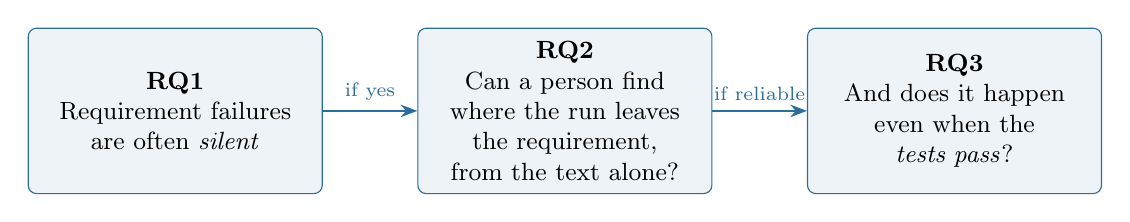
\begin{tikzpicture}[
      box/.style={draw=accentBlue, fill=accentBlue!8, rounded corners=3pt, align=center,
                  minimum height=2.1cm, text width=3.5cm, font=\small, execute at begin node={\hyphenpenalty=10000\exhyphenpenalty=10000}},
      arr/.style={-{Stealth[length=6pt]}, thick, accentBlue}]
    \node[box] (r1) {\textbf{RQ1}\\ Requirement failures\\ are often \emph{silent}};
    \node[box, right=1.2cm of r1] (r2) {\textbf{RQ2}\\ Can a person find\\ where the run leaves\\ the requirement,\\ from the text alone?};
    \node[box, right=1.2cm of r2] (r3) {\textbf{RQ3}\\ And does it happen\\ even when the\\ \emph{tests pass}?};
    \draw[arr] (r1) -- node[above, font=\scriptsize]{if yes} (r2);
    \draw[arr] (r2) -- node[above, font=\scriptsize]{if reliable} (r3);
  \end{tikzpicture}
  \vspace{10pt}
  \begin{itemize}\small
    \item Bridge version: RQ1 shows alarms miss wrong-island bridges; RQ2 asks whether an inspector with the contract
      can point to the exact spot; RQ3 asks whether bridges that \emph{passed} inspection still go to the wrong island.
    \item A failing test shows a problem; a passing test does not prove the requirement was met.
  \end{itemize}
  \note{If RQ1 shows no silence gap, RQ2 and RQ3 still stand but need a different motivation; we would say so.}
\end{frame}

% =====================================================================
\section{Plan}

\begin{frame}{This week (Sep 28 -- Oct 4)}
  \small
  \begin{tabularx}{\textwidth}{@{}llL@{}}
    \toprule
    \textbf{When} & \textbf{Who} & \textbf{What} \\
    \midrule
    Mon & Cris & Send video + this deck; send Kundi the guide and his 50 runs \\
    Mon--Tue & Cris & Finish labeling the remaining 381 runs \\
    Mon--Wed & Kundi & Label 50 runs blind ($\sim$1 hour) \\
    Wed & Cris + Claude & Agreement script; fix guide if needed; \textbf{freeze the plan} \\
    Thu & Claude & Run the comparison: table, redraws, four checks \\
    Fri & Cris & Write RQ1 findings; pick the Nebius sample and write the silence rule \\
    \bottomrule
  \end{tabularx}
  \note{The only blocking items are the 381 labels and Kundi's 50.}
\end{frame}

\begin{frame}{Road to the deadline}
  \small
  \begin{tabularx}{\textwidth}{@{}lL@{}}
    \toprule
    \textbf{Dates} & \textbf{Milestone} \\
    \midrule
    Sep 28 -- Oct 4 & RQ1 Study 1 (FaaP) done \\
    Oct 5 -- Oct 23 & Study 2 (Nebius, $\sim$200 runs); RQ2 and RQ3 on Nebius Draw 2 \\
    Oct 24 -- Nov 1 & Write the paper; \textbf{abstract due Nov 1} \\
    Nov 1 -- Nov 6 & Polish; \textbf{paper due Nov 6 (AoE)}; full paper, 8 pages incl.\ references \\
    \bottomrule
  \end{tabularx}
  \vspace{6pt}
  \begin{block}{What we need from you}\small
    \textbf{Kundi:} label the 50 blind runs.
    \textbf{Kundi and Sanaa:} agree with the two labeling rules? Confirm RQ2 and RQ3 wording.
  \end{block}
  \note{Tight but doable if Study 2 stays around 200 runs. Fallback per Kundi: 4-page short paper.}
\end{frame}

\end{document}
